\documentclass{beamer}
%\usetheme{Ilmenau}
%\usecolortheme{beaver}

\usepackage[slovak,american]{babel}
\usepackage[utf8]{inputenc}
\usepackage{graphicx}
\usepackage{adjustbox}
\usepackage{xcolor}
\usepackage{mathrsfs}
 
 \newsavebox\MBox
\newcommand\Cline[2][red]{{\sbox\MBox{$#2$}%
  \rlap{\usebox\MBox}\color{#1}\rule[-2.2\dp\MBox]{\wd\MBox}{1pt}}}

%\usefonttheme{serif}

%\definecolor{UKOrange}{HTML}{ef9424} %
\definecolor{UKOrange}{HTML}{7a2c18} %
\definecolor{UKBrown}{HTML}{a96d5e} %
\definecolor{UKLight}{HTML}{d8b6ab} %
\definecolor{UKDark}{HTML}{7a4f44}
\definecolor{UKDarker}{HTML}{4d312b} 
\definecolor{UKDarkest}{HTML}{2e1e1a}
\definecolor{UKRed}{HTML}{bf1f1c}

\setbeamertemplate{footline}[frame number]{}
\setbeamertemplate{navigation symbols}{}

%\usecolortheme{beaver}
\setbeamertemplate{itemize item}[square]
\setbeamercolor{itemize item}{fg = UKBrown}
\setbeamercolor{itemize subitem}{fg = UKLight}
\setbeamercolor{enumerate item}{fg = UKDark}

\setbeamercolor{footnote}{fg=UKLight}
\setbeamercolor{footnote mark}{fg=UKLight}
\setbeamerfont{footnote}{size=\tiny}
\renewcommand\footnoterule{}

\usetheme{default}
\beamertemplatenavigationsymbolsempty
\setbeamercolor{title}{fg=white, bg=UKBrown}
\setbeamercolor{frametitle}{fg=white, bg=UKBrown}
\setbeamercolor{block title}{bg=UKBrown, fg= white}
\setbeamercolor{block body}{bg =UKLight, fg = UKDarkest}

\setbeamercolor{block title alerted}{bg=UKOrange, fg= white}
\setbeamercolor{block body alerted}{bg =UKLight, fg = UKDarkest}


%\setbeamercolor{section in toc}{fg = UKBrown}
%\setbeamercolor{section in toc}{fg = UKDarkest}

% odstrani gulicky
\renewcommand*{\slideentry}[6]{}

\useoutertheme[subsection=false]{miniframes}
\AtBeginSection[]{\subsection{}}

\setbeamercolor{below lower separation line head}{bg=UKDark}
\addtobeamertemplate{headline}{}{%
  \begin{beamercolorbox}[colsep=0.5pt]{below lower separation line head}
  \end{beamercolorbox}
}
%\setbeamercolor*{mini frame}{fg=white,bg=UKRosy}
\setbeamercolor{section in head/foot}{fg=UKLight, bg=UKDark}

\usepackage{etoolbox}
\makeatletter
\preto{\@verbatim}{\topsep=0pt \partopsep=0pt }
\makeatother

%\setbeamertemplate{itemize/enumerate body begin}{\normalsize}
%\setbeamertemplate{itemize/enumerate subbody begin}{\normalsize}




%\newcommand{\codeblock}[2]{ \begin{block}{#1} \begin{verbatim}#2\end{verbatim}\end{block}}

%\defbeamertemplate*{title page}{customized}[1][]
%{
%  \begin{centering}
%    \begin{beamercolorbox}[sep=8pt,center]{title}
%      \usebeamerfont{title}\inserttitle
%    \end{beamercolorbox}
%  \end{centering}
%  \bigskip
%
%\begin{columns}[onlytextwidth,T]
%
%
%  \column{27mm}
%  \includegraphics[width=27mm]{images/logoFMFI.png}
%  
%  \column{\dimexpr\linewidth-54mm-6mm}
%  \centering
%  \vspace{5mm}  
%  \usebeamerfont{author}\insertauthor\par
%  \vspace{5mm}
%  \usebeamerfont{institute}\insertinstitute\par
%
%  \column{27mm}
%  \includegraphics[width=27mm]{images/logoUK.png}  
%\end{columns}
%\centering
%\vspace{7mm}
%  \usebeamerfont{date}\insertdate\par
%}

\DeclareMathOperator*{\argmin}{arg\,min}
\newcommand{\e}[1]{$\cdot 10^{#1}$}

%\newcommand{\codeblock}[2]{ \begin{block}{#1} \begin{verbatim}#2\end{verbatim}\end{block}}



\title[11. cvičenie]{Pokročilé spracovanie obrazu - Transformácie Obrazu}
\author[Kocur]{Ing. Viktor Kocur \\{\small viktor.kocur@fmph.uniba.sk}}
\institute{DAI FMFI UK}
\date{4.12.2019}

\begin{document}
\selectlanguage{slovak}

\begin{frame}

  \titlepage

\end{frame}

\section{Zmena veľkosti obrazu}


\begin{frame}
\frametitle{Informácia v obraze}
\centering
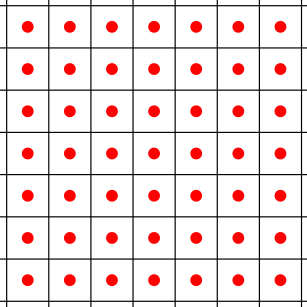
\includegraphics[width=0.6\textwidth]{resize1.png}\\

Uvažujeme, že informácia o intenzite je v strede pixela.
\end{frame}


\begin{frame}
\frametitle{Informácia v obraze}
\centering
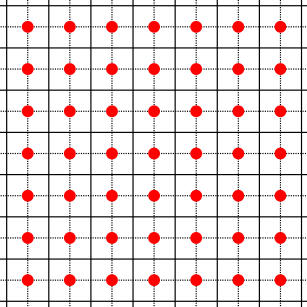
\includegraphics[width=0.6\textwidth]{resize2.png} \\
Prerušovaná mriežka nám teda nerozdeuje hranicu medzi pixelmi, ale určuje stredy pixelov.
\end{frame}

\begin{frame}
\frametitle{Informácia v obraze}
\centering
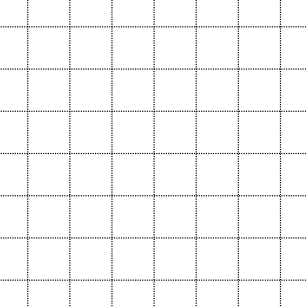
\includegraphics[width=0.6\textwidth]{resize3.png}
\end{frame}


\begin{frame}
\frametitle{Zväčšenie obrazu}
\centering
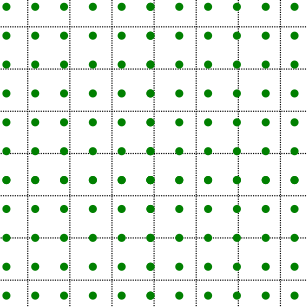
\includegraphics[width=0.6\textwidth]{resize4.png}
\end{frame}


\begin{frame}
\centering
\frametitle{Zmenšenie obrazu}
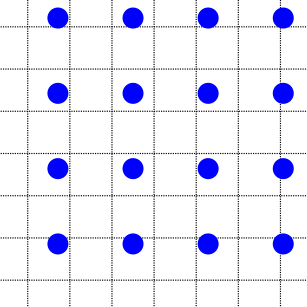
\includegraphics[width=0.6\textwidth]{resize5.png}
\end{frame}

\begin{frame}
\centering
\frametitle{Interpolácia}
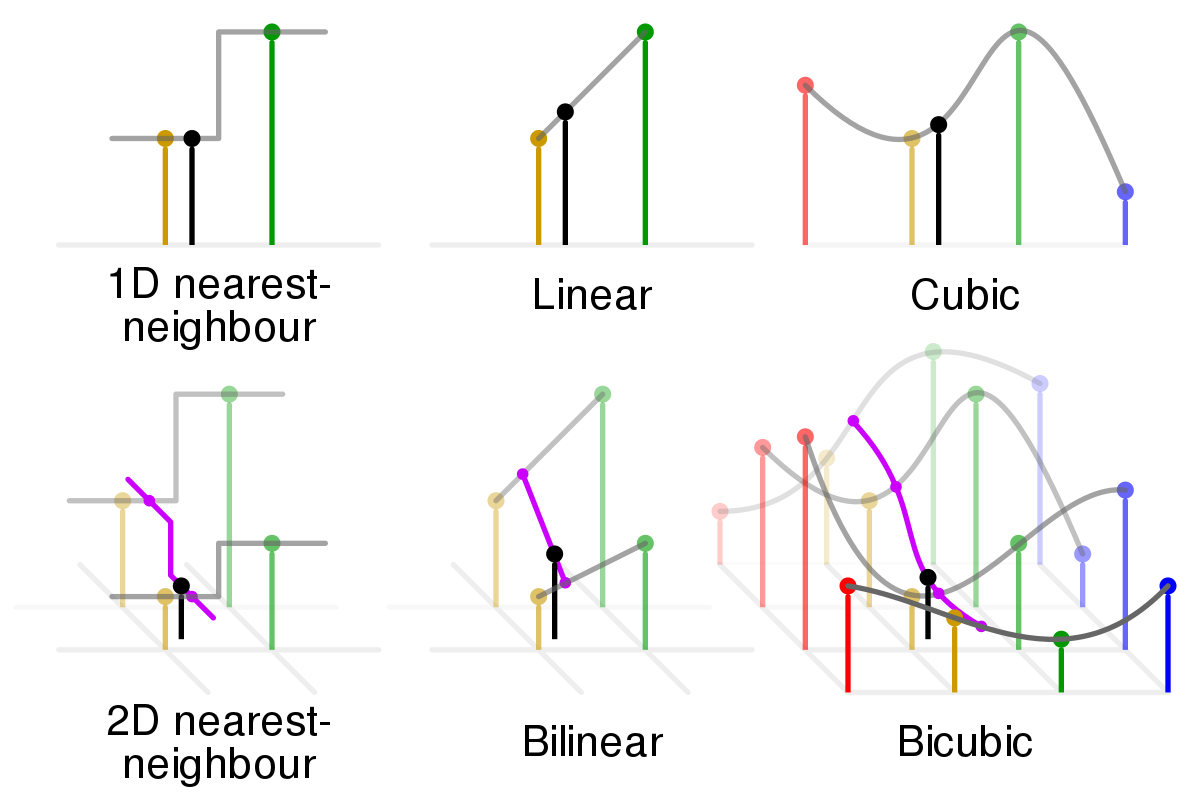
\includegraphics[width=0.8\textwidth]{interpolation.png} \\
To aké hodnoty budú mať pixely po operácii rátame pomocou interpolácie z pixelov v okolí umiestnenia nového bodu.
\end{frame}


\begin{frame}
\centering
\frametitle{Zmena veľkosti v Matlabe}
\begin{block}{imresize}
imresize(I, scale) - vráti obraz po zväčšení škálovacím faktorom scale
\end{block}

\begin{block}{imresize}
imresize(I, [r, c]) - vráti obraz po zväčšení na rozmer $r \times c$
\end{block}

\begin{block}{imresize}
imresize(I, s, 'method') - vráti obraz po zväčšení, ale s použitím metódy z 'nearest', 'bilinear', 'bicubic'.
\end{block}

\begin{block}{Úloha}
Otestujte si imresize s rôznymi metódami pre zväčšnie shell.png a zmenšenie zátišia.
\end{block}
\end{frame}

\section{Transformácia obrazu}

\begin{frame}
\centering
\frametitle{Afinná transformácia}
\begin{block}{Ako sa počíta}
Transformáciu počítame pomocou zápisu kde $\vec{y}$ predstavuje novú polohu daného pixela.
$$ \vec{y} = \mathbb{A}\vec{x} + \vec{t}$$
\end{block}

\begin{alertblock}{Využitie v obraze}
V obraze nepočítame nové polohy $\vec{y}$ na základe existujúcich polôh stredov pixelov $\vec{x}$, ale najprv si určíme nejakú rovnomernú množinu pre body $\vec{y}$ a potom inverzne spočítame k nim body $\vec{x} = \mathbb{A}^{-1} (\vec{y} -\vec{t})$. To nám umožní jednoducho opäť použiť interpoláciu pre body v obraze. 
\end{alertblock}
\end{frame}

\begin{frame}
\centering
\frametitle{Príklady}
\begin{block}{Rotácia}
$$ \mathbb{A} = \begin{bmatrix}
    cos(\alpha)       & -sin(\alpha)  \\
    sin(\alpha)       & cos(\alpha)  \\   
\end{bmatrix}$$
\end{block}

\begin{block}{Natiahnutie po x-ovej osi}
$$ \mathbb{A} = \begin{bmatrix}
    2       & 0  \\
    0       & 1  \\   
\end{bmatrix}$$
\end{block}
\end{frame}

\begin{frame}
\centering
\frametitle{Rotácia}

\includegraphics[width=0.6\textwidth]{rotate.png}
\end{frame}

\begin{frame}
\centering
\frametitle{Afinná transformácia}

\includegraphics[width=0.6\textwidth]{afine.png}
\end{frame}


\begin{frame}
\frametitle{Afinná transformácia v Matlabe}
\begin{block}{imtransform}
imtransform(I, tform, interp) - transfomuje obraz I podľa transformačného objektu tform pomocou interpolačnej metódy interp: z 'nearest', 'bilinear', 'bicubic'.
\end{block}

\begin{block}{maketform}
maketform('affine', B) - vráti transformačný objekt pre afinnú transformáciu. Afinná transformácia je definovaná maticou B, ktorá sa skladá s našej matice A s pridaným stĺpcom s vektorom $\vec{t}$.
\end{block}

\begin{block}{imrotate}
imrotate(I, angle) - vráti orotovaný obrázok I o uhol angle.
\end{block}
\end{frame}


\begin{frame}
\frametitle{Úlohy}
\begin{block}{Úloha}
Urobte rotáciu obrázku pomocou imrotate. Skúste urobiť rotáciu aj pomocou afinnej transformácie.
\end{block}

\begin{block}{Úloha}
Vytvorte afinnú transformáciu ktorá prehodí obraz len po x-ovej ose, alebo len po y-vej ose.
\end{block}

\begin{block}{Úloha}
Otestujte si rôzne matice pre afinnú transformáciu.
\end{block}
\end{frame}


\begin{frame}
\frametitle{Perspektívna transformácia}
\begin{block}{imtransform}
imtransform(I, tform, interp) - transfomuje obraz I podľa transformačného objektu tform pomocou interpolačnej metódy interp: z 'nearest', 'bilinear', 'bicubic'.
\end{block}

\begin{block}{maketform}
maketform('projective', U, X) - vráti transformačný objekt pre perspektívnu transformáciu. Matice U a X majú tvar $4 \times 2$. Každý riadok matice U je transformovaný na korešpondujúci riadok matice X. 
\end{block}

\begin{block}{Matice U a X}
Maticu U môžeme vyrobiť pomocou volania U = ginput(4). Rovnako môžeme vyrobiť aj maticu X, alebo ak chceme napr. obraz rektifikovať (zarovnať s osami) tak si vyrobíme maticu ktorá na každom riadku bude mať pozíciu rohu obdĺžnika.
\end{block}
\end{frame}


\begin{frame}
\frametitle{Úlohy}
\begin{block}{Úloha}
V obrázku qr.jpg použite perspektívnu transformáciu tak, aby boli QR kódy zarovnané s osami. Podobne zarovnajte aj obrázok book.jpg.
\end{block}

\begin{block}{Úloha}
V obrázku road.png použite perspektívnu transformáciu tak, aby boli vodiace čiary zarovnané s y-ovou osou. Je toto zadanie jednoznačné z hľadiska výsledného obrazu?
\end{block}
\end{frame}




\end{document}